\chapter{Models, Views and Templates}

Models, views and templates consist the core of Teakwood System. The majority coding in Teakwood happens here. Models generate all the database tables; View provides all the web page functions; and templates generate all the HTML files. In an operational degree of view, models response for communicating with data; View decides which data to display; and templates decorate the data for displaying.

\begin{figure}[htb]
\centering
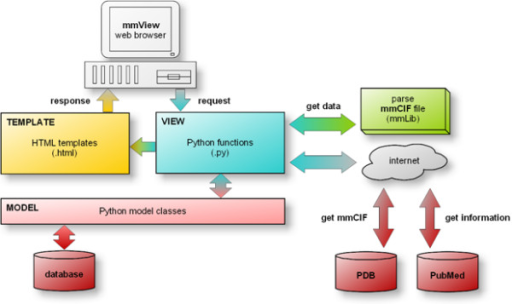
\includegraphics[scale=0.7]{./mtv}
\caption{Teakwood MTV Framework}
\label{fig:label} % insert suitable label, this is used to refer to a fig from within the text as shown above
\end{figure}

As we can see from the figure, Teakwood has a loose coupled modeling design. model, view, and template are separated from each other; each application(The light green square) is also separated from each other. This design makes the Teakwood system flexible to make changes and easy to extend feathers.

\section{Models and Database}

The models are Python objects that describes Teakwood data models/tables. Thanks to the system integrated object relational mapping (ORM) functions, I don't have work with SQL database in order to manipulate data; all we should do is manipulating the corresponding Python objects, ORM will do the mapping work.\\

For example this section of python code:
\begin{verbatim}
class Person(models.Model):
    first_name = models.CharField(max_length=30)
    last_name = models.CharField(max_length=30)
\end{verbatim}

will generate a database table like this:
\begin{verbatim}
CREATE TABLE myapp_person (
    "id" serial NOT NULL PRIMARY KEY,
    "first_name" varchar(30) NOT NULL,
    "last_name" varchar(30) NOT NULL
);
\end{verbatim}

So for the database designing what I did is create the "models.py" files and define the corresponding classes for mapping.

\section{Views functions}
The View layer are Python functions that defining Teakwood business logic. For example if I want to show my user information, I have  to write a view function to tell the model layer pulling the User data from database I also have to decide which template.html be used for data decorating. As such, I will have to define two logic functions in my views.py file. In general, View layer can be seeing as a bridge between the model and the template. \\

Take a look at this example in Teakwood job view models.
\begin{verbatim}
@login_required
def job_view(request, job_id):
    job = get_object_or_404(Job, pk=job_id)

    if request.user == job.user or 
    request.user.groups.filter(name=job.group):
        return render_to_response
        ('simfactory/job_detail.html',
        {'object': job},
        context_instance=RequestContext(request))
    else:
        return redirect(reverse("simfactory_joblist"))
\end{verbatim}

This code will execute when I click your job-view button on my job console. It tells the model layer to pull the job information if the user is authenticated, otherwise redirect to job list.

\section{Template Language}

Teakwood’s template language is designed to strike a balance between power and ease. It is designed to please both the HTML designer and the Python coder. Teakwood template language is not just HTML files or Python code. Here is an example:\\

\begin{verbatim}

{{ section.title }}

<h1>{{ section.title }}</h1>

<h2><a href="{{ story.get_absolute_url }}">
    {{ story.headline|upper }}
  </a></h2>
<p>{{ story.tease|truncatewords:"100" }}</p>


\end{verbatim}

We can see there are some special symbols in the HTML code. Basically there are three types of special symbols in Teakwood template language: variables, tags and filters.\\

\textbf{Variable}: When the template engine encounters a variable, it evaluates that variable and replaces it with the result.\\
\textbf{Tag }: Tags are more complex than variables: Some create text in the output, some control flow by performing loops or logic, and some load external information into the template to be used by later variables. Some tags require beginning and ending tags. \\
\textbf{filter}:Filter is basically a restricted variable.\\

With the help of variables and tags, static HTML files become dynamic HTML files and can interact with python code.

Template files in template directory generate all the visible HTML content for Teakwood system. There are roughly 100 template files in Teakwood, all of them have to be predefined and wait for the calling from View.
